\chapter{Automatización}
\label{chap:automation}


\section{Introducción}

En este capítulo se describen procesos de automatización y se realizará un análisisi del código de todas las partes del asistente virtual (backend, frontend y python). Se realizarán test unitarios

\section{Estado actual}

Actualmente, el sistema del asistente virtual no tiene ningún tipo de automatización u otro mecanismo de análisis de código. 

\begin{itemize}
    \item Análisis de código: No se ha realizado ningún análisis de código durante el desarrollo ni la la puesta en el entorno de producción para las pruebas del cliente. No se ha barajado incluir una herramienta de análisis de código dentro del proceso de desarrollo.
    \item Pruebas (integración y funcionales): No se han tenido en cuenta ningún tipo de pruebas, ni funcionales, ni de integración.
    \item CI/CD: No se hace uso de ningún tipo de softwares o plataformas de integración continua y despliegue continuo. El equipo trabaja con Bitbucket, pero no ha utilizado ningún plugin o software relativo para ello.
\end{itemize}






\section{Problemas encontrados}

Analizando el estado actual de la herramienta se pueden observar los siguientes problemas:

\begin{itemize}
    \item Pruebas: Dado que el equipo no hace uso de un entorno de pruebas o preproducción, si no que directamente despliega la aplicación del entorno de desarrollo al entorno de producción, no se realizan pruebas sobre el despliegue del sistema. Además, se ha observado que no se realizan pruebas funcionales ni análisis de código durante el desarrollo.
    \item Malas prácticas: El equipo utiliza Bitbucket como repositorio pero carece de una guía o de un sistema para subir al entorno de produccion. No se hace uso de herramientas de integración continua o despliegue continuo.
    \item Calidad del software: Se ha realizado un análisis estático del repositorio con el sistema del asistente mediante SonarCloud. Este análisis nos ofrece una visión global del estado actual del proyecto.
\end{itemize}

Para el análisis estático y tests se ha utilizado SonarCloud. En la figura 6.1 se puede observar el resumen del análisis y, teniendo en cuenta que es un proyecto que se encuentra desplegado en un entorno de producción, destaca que no se han encontrado ningún error de seguridad (si revisiones), pero si se han encontrado 2 bugs importantes (en el icono del frontend del asistente virtual y en un método de /controller).
\newpage

\begin{figure}[h]
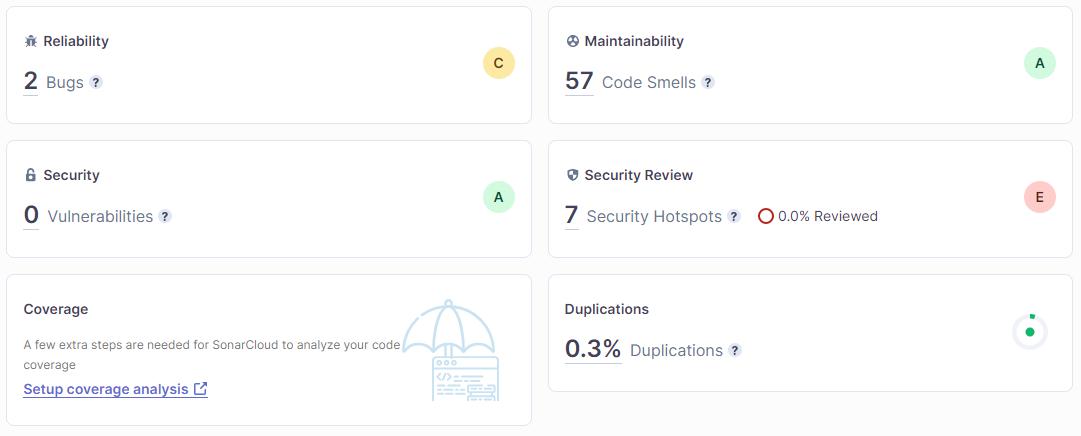
\includegraphics[width=\textwidth]{figures/Overview-code.png}
\caption{Resumen del análisis realizado por SonarCloud}
\label{fig:esquema}
\end{figure}



En la figura 6.2 se pueden ver en detalle los dos bugs mencionados:

\begin{figure}[h]
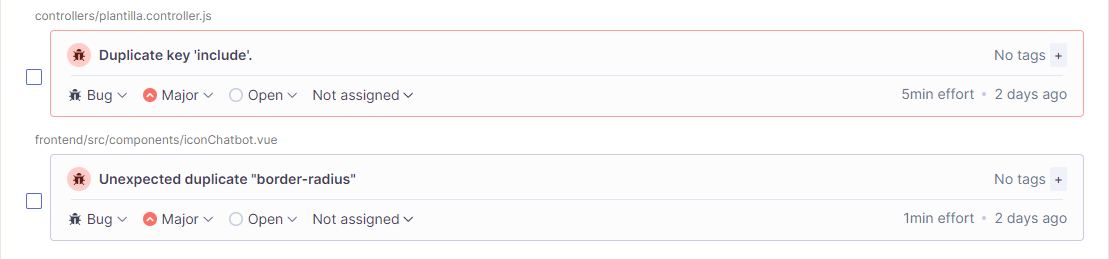
\includegraphics[width=\textwidth]{figures/bug-example.png}
\caption{Ejemplos de bugs en el proyecto}
\label{fig:esquema}
\end{figure}


A pesar de que el análisis en SonarCloud no ha encontrado grandes problemas o vulenerabilidades en el código desde un punto de vista de seguridad, es importante destacar que todo este desarrollo se ha realizado sin haber tenido en cuenta estas herramientas y por errores humanos se pueden generar vulnerabilidades. Este tipo de análisis prorpociona un apoyo.

En una vista más detallada por carpetas (estructura) del proyecto, figura 6.3, se pueden observar la distribución de estas vulnerabilidades detectadas en el código. Destaca la existencia de código duplicado sobre todo en el backend.

\newpage

\begin{figure}[h]
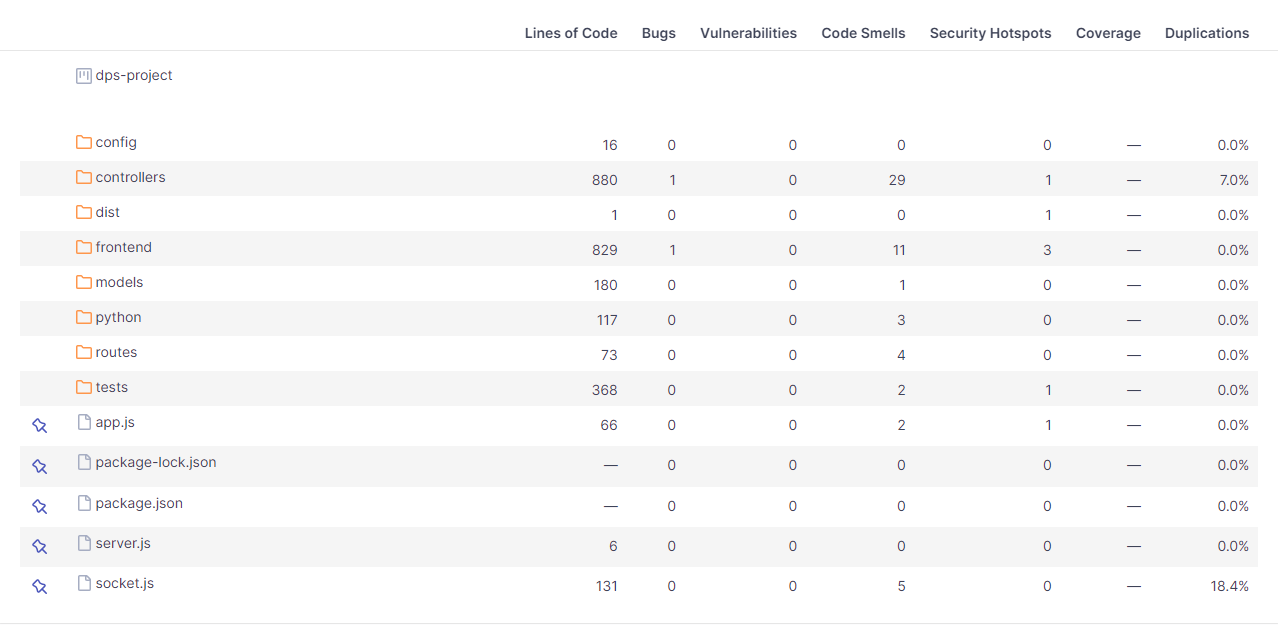
\includegraphics[width=\textwidth]{figures/Code-issues.png}
\caption{Detalle del código con las vulnerabilidades obtenidas por SonarCloud}
\label{fig:esquema}
\end{figure}







\section{Soluciones propuestas}

Teniendo en cuenta los problemas mencionados y el estado actual, se proponen las siguientes medidas:

\begin{itemize}
    \item Pruebas (integración y funcionales): El equipo de desarrollo debería realizar pruebas a corto plazo ya que ahora mismo no se desarrollan.
    \item Análisis de la calidad del código: Se propone que se realicen buenas prácticas de análisis de código para comprobar vulnerabilidades que puedan surgir durante el desarrollo y despliegue del proyecto. 
    \item Integración y Despliegue continuo (CI/CD): Se propone utilizar herramientas destinadas a este propósito. Estas herramientas ayudan al equipo de desarrollo y son un apoyo a la hora de detectar vulnerabilidades, además que son buenas prácticas.
    
\end{itemize}